\documentclass[
    12pt,                % tamanho da fonte
    openright,           % capítulos começam sempre em página ímpar
    oneside,             % impressão só frente (use "twoside" se frente e verso)
    a4paper,             % papel A4
    brazil               % idioma principal
]{abntex2}

% Pacotes básicos
\usepackage[utf8]{inputenc}   % acentuação
\usepackage[T1]{fontenc}      % codificação da fonte
\usepackage{lmodern}          % usa fonte Latin Modern
\usepackage{microtype}        % melhora a justificação
\usepackage{graphicx}         % inserir figuras
\usepackage{abntex2cite}      % citações padrão ABNT
\usepackage{url}  
\usepackage{indentfirst}       % recuo no primeiro parágrafo
\usepackage{ragged2e}          % para justificação
\usepackage{amsmath} % para \text{} e outras paradas de equação
\usepackage{multirow} %para o multirow
\usepackage{float} % necessário para [H]
\usepackage{pgfplots}


% Recuo e espaçamento entre parágrafos (ABNT)
\setlength{\parindent}{1.25cm} % recuo de 1,25 cm
\setlength{\parskip}{0.2cm}    % espaço entre parágrafos

% Informações do trabalho
\titulo{Título do seu TCC}
\autor{João Victor Sousa}
\local{Ilhéus - Bahia}
\data{2025}
\orientador{Otacílio José Pereira}
\instituicao{
  Universidade Estadual de Santa Cruz \par
  Curso de Graduação em Ciênca da Computação}
\tipotrabalho{Trabalho de Conclusão de Curso}
\preambulo{Trabalho apresentado ao Curso de Y da Universidade X como requisito parcial para obtenção do título de Bacharel.}

\begin{document}

% Capa e folha de rosto
\imprimircapa
\imprimirfolhaderosto*

% Resumo
\begin{resumo}
Escreva aqui o resumo do seu trabalho.  
Inclua objetivos, metodologia, resultados e conclusões.

\vspace{\onelineskip}
\noindent
\textbf{Palavras-chave}: palavra1. palavra2. palavra3.
\end{resumo}

% Sumário
\tableofcontents

%chapt* é um captulo sem numeração
\chapter*{Lista de Siglas} 
\begin{tabular}{ll}
AUC & Area Under Curve \\
RNN & Redes Neurais Recorrentes \\
CNN & Redes Neurais Convolucionais \\
LSTM & Long Short-Term Memory \\
AAMI & Association for the Advancement of Medical Instrumentation   \\
GRU & Gated Unit Recurrent \\
ECG & Eletrocardiograma \\
TP & Verdadeiro Positivo \\
FP & Falso Positivo \\
TN & Verdadeiro Negativo \\
FN & Falso Negativo \\
\end{tabular}



% Capítulos
\chapter{Introdução}
Texto da introdução.

\chapter{Metodologia}

Primeiramente, foi necessário definir qual banco de dados seria utilizado para o treinamento e a validação. Optou-se pelo \textit{MIT-BIH Arrhythmia Database} \cite{mitbih2005}, recomendado pela AAMI. O banco é composto por 58 registros de eletrocardiograma (ECG), cada um com 30 minutos de duração. Os 23 primeiros registros foram selecionados aleatoriamente a partir de um conjunto de 4000 gravações de 24 horas realizadas em pacientes ambulatoriais do Beth Israel Deaconess Medical Center. Os 25 registros restantes foram escolhidos de modo a incluir arritmias raras, mas clinicamente significativas.

Uma característica importante desse banco é a anotação de cada batimento cardíaco em torno do complexo R, realizada por três cardiologistas independentes.

\section{Particionamento dos dados e classes}

Os dados foram particionados seguindo a estratégia inter-paciente proposta por Chazel et al. (apud \citeonline{silva2025}), na qual batimentos de um mesmo paciente não podem aparecer simultaneamente nos conjuntos de treinamento e validação. O objetivo é garantir a capacidade de generalização do modelo para diferentes pacientes. Além disso, conforme recomendado pela AAMI, registros de pacientes com marcapasso foram excluídos.  

Os registros 101, 106, 108, 109, 112, 114, 115, 116, 118, 119, 122, 124, 201, 203, 205, 207, 208, 209, 215, 220, 223 e 230 foram utilizados para treinamento (conjunto DS1). Os demais (100, 103, 105, 111, 113, 117, 121, 123, 200, 202, 210, 212, 213, 214, 219, 221, 222, 228, 231, 232, 233 e 234) formaram o conjunto de teste (DS2).

De acordo com a AAMI (apud \citeonline{silva2025}), são definidas cinco classes de arritmia: N, SVEB, VEB, F e Q, correspondentes a batimento normal, batimento supraventricular ectópico, batimento ventricular ectópico, fusão de batimento ventricular e normal e batimento não classificado, respectivamente. A Tabela~\ref{tab:particionamento} apresenta a distribuição dessas classes no conjunto de dados.

\begin{table}[htb]
\centering
\caption{Particionamento inter-paciente proposto por Chazel et al.}
\label{tab:particionamento}
\begin{tabular}{|l|c|c|c|c|c|c|}
\hline
Conjunto & N & SVEB & VEB & F & Q & Total \\ \hline
DS1 & 45 866 & 944 & 3 788 & 415 & 8 & 51 021 \\ \hline
DS2 & 44 259 & 1 837 & 3 221 & 388 & 7 & 49 712 \\ \hline
Total & 90 125 & 2 781 & 7 009 & 803 & 15 & 100 733 \\ \hline
\end{tabular}
\legend{Fonte: Adaptado de Silva et al. (2025).}
\end{table}

O conjunto DS1 foi então subdividido em treinamento e validação por meio de validação cruzada, inicialmente com duas partições (dois \textit{folds}) e, posteriormente, com cinco partições (cinco \textit{folds}) nos modelos finais.  

Considerando o desbalanceamento dos dados e visando maior simplicidade, adotou-se a classificação binária, na qual a classe positiva corresponde a arritmia e a classe negativa a batimentos normais.

\section{Métricas}

As métricas utilizadas para avaliar o desempenho dos modelos foram: sensibilidade, precisão, acurácia, \textit{F1-score} e AUC (\textit{Area Under the Curve}).  

A sensibilidade representa a capacidade do modelo em identificar corretamente as classes positivas, isto é, os batimentos arrítmicos. Sua equação é dada por:

\begin{equation}
\text{Sensibilidade} = \frac{TP}{TP + FN}
\end{equation}

em que $TP$ são os verdadeiros positivos e $FN$ os falsos negativos.  

A precisão, por sua vez, indica a proporção de batimentos classificados como arrítmicos que realmente pertencem a essa classe:

\begin{equation}
\text{Precisão} = \frac{TP}{TP + FP}
\end{equation}

onde $FP$ representa os falsos positivos. Precisão e sensibilidade estão relacionadas por um \textit{trade-off}. No contexto médico, prioriza-se elevada sensibilidade, ainda que à custa de menor precisão, uma vez que falsos negativos são mais prejudiciais que falsos positivos.  

O \textit{F1-score} é a média harmônica entre precisão e sensibilidade, buscando um equilíbrio entre ambas:

\begin{equation}
\text{\textit{F1-score}} = \frac{2 \cdot \text{Precisão} \cdot \text{Sensibilidade}}{\text{Precisão} + \text{Sensibilidade}}
\end{equation}

A acurácia corresponde ao acerto global do modelo, considerando tanto as classes positivas quanto as negativas:

\begin{equation}
\text{Acurácia} = \frac{TP + TN}{TP + TN + FP + FN}
\end{equation}

A AUC mede a capacidade do modelo em separar as classes positivas das negativas, variando entre 0 e 1. Valores próximos de 1 indicam separação perfeita, enquanto 0,5 corresponde a um modelo com desempenho equivalente ao acaso. 

Essa métrica é calculada a partir da área sob a curva ROC, ilustrada na Figura~\ref{fig:roc}.


\begin{figure}[H]
    \centering
    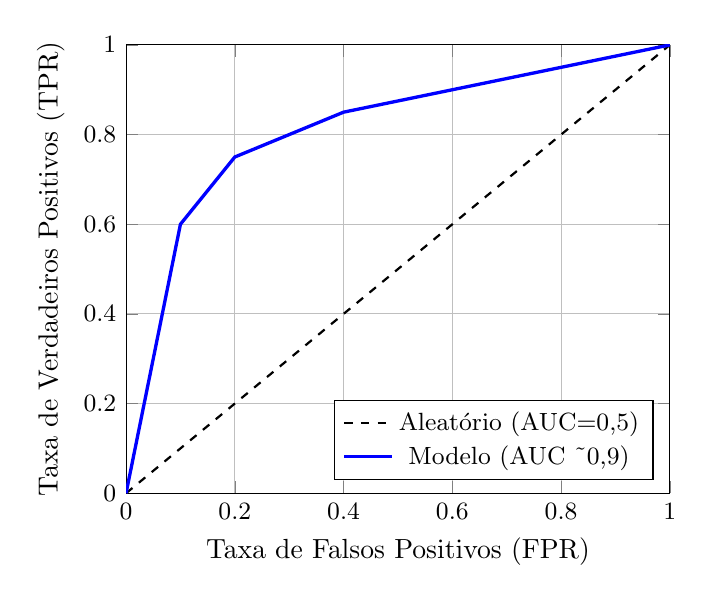
\begin{tikzpicture}
        \begin{axis}[
            width=0.7\textwidth,
            height=0.6\textwidth,
            grid=both,
            xlabel={Taxa de Falsos Positivos (FPR)},
            ylabel={Taxa de Verdadeiros Positivos (TPR)},
            xmin=0, xmax=1,
            ymin=0, ymax=1,
            legend pos=south east,
            legend style={font=\small},
            tick label style={font=\small}
        ]

        % Linha do classificador aleatório
        \addplot[domain=0:1, dashed, thick, color=black] {x};
        \addlegendentry{Aleatório (AUC=0,5)}

        % Curva ROC simulada
        \addplot[color=blue, very thick] coordinates {
            (0,0)
            (0.1,0.6)
            (0.2,0.75)
            (0.4,0.85)
            (0.6,0.9)
            (0.8,0.95)
            (1,1)
        };
        \addlegendentry{Modelo (AUC \textasciitilde 0,9)}

        \end{axis}
    \end{tikzpicture}
    \caption{Exemplo de curva ROC: comparação entre modelo aleatório e modelo com bom desempenho.}
    \label{fig:roc}
\end{figure}

A matriz de confusão, por fim, fornece uma representação tabular dos acertos e erros do modelo, como exemplificado na Tabela~\ref{tab:matriz_confusao}.

\begin{table}[H]
\centering
\caption{Exemplo de matriz de confusão binária}
\label{tab:matriz_confusao}
\begin{tabular}{|c|c|c|}
\hline
\multirow{2}{*}{\textbf{Classe Verdadeira}} & \multicolumn{2}{c|}{\textbf{Classe Predita}} \\ \cline{2-3} 
 & Positiva & Negativa \\ \hline
Positiva & TP & FN \\ \hline
Negativa & FP & TN \\ \hline
\end{tabular}
\legend{Fonte: Elaborado pelo autor.}
\end{table}

Essas métricas em conjunto permitem avaliar não apenas a proporção global de acertos, mas também a capacidade do modelo em detectar corretamente arritmias, aspecto essencial em aplicações médicas.


\section{Modelos utilizados}

Como o diagnóstico de arritmias depende tanto do aspecto morfológico dos ECGs quanto do aspecto sequencial, isto é, o ritmo, foram escolhidos modelos RNNs que possuem
bom desempenho em dados sequenciais como séries temporais e linguagem natural \cite{james2023}. Já as redes CNN possuem grande capacidade de extração de características
e podem aprender os aspectos morfológicos dos ECGs. 



\section{Organização da entrada}

Foi escolhido de cada ECG o lead MLII que facilita a visualização do complexo QRS. Quando disponível. 
O ECG foi limpo utilizando a biblioteca neurokit2.

Cada batimento foi segmentado utilizando a bibliteca neurokit2 \cite{Makowski2021neurokit}.
Com os batimentos segmentados foi montado uma matriz tridimensional no formato: (\textit{batch size}, tamanho da sequência, características). As características inicialmente correspondem as amostras do ECGs e demais 
características como intervalo RR, média do intervalo RR para o paciente e a média do 5 intervalos RR anteriores e posteriores. Em cada sequência de batimentos, só há batimentos exclusivos de um
único paciente.



\chapter{Resultados}
Texto dos resultados.

\chapter{Conclusão}
Texto da conclusão.

% Referências (BibTeX)
\bibliographystyle{abntex2-alf}
\bibliography{referencias}

\end{document}
